\documentclass[a4paper,10pt]{article}
%\documentclass[a4paper,10pt]{scrartcl}

\usepackage[utf8]{inputenc}
\usepackage{amsmath}
\usepackage{listings}
\usepackage{hyperref}
\usepackage{catoptions}
\usepackage[margin=1in]{geometry}
\usepackage{color}
\usepackage{soul}
\usepackage{float}
\usepackage{framed}
\usepackage[sc]{mathpazo}
\linespread{1.20}         % Palatino needs more leading (space between lines)
\usepackage[T1]{fontenc}
\usepackage{microtype}
\usepackage{enumerate}
\usepackage{courier}
\usepackage{graphicx}

\newcommand{\authorbd}{Bas Dado (4033736)}
\newcommand{\authoroh}{Olivier Hokke (1352679)}
\newcommand{\authortr}{Tom Runia (1517996)}
\newcommand{\authoras}{Arnold Schutter (?)}
\newcommand{\authortv}{Tom Viering (4333055)}
\newcommand{\maintitle}{IN4010: Negotiation Project}
\newcommand{\subtitle}{Group 7 - BOAconstructor}

\title{\maintitle\\\subtitle}
\author{\authorbd\\\authoroh\\\authortr\\\authoras\\\authortv}
\date{\today}

\pdfinfo{%
  /Title    (\maintitle - \subtitle)
  /Author   (\authorbd, \authoroh, \authortr, \authoras, \authortv)
  /Creator  (\authorbd, \authoroh, \authortr, \authoras, \authortv)
  /Producer (\authorbd, \authoroh, \authortr, \authoras, \authortv)
  /Subject  (Automated Negotiation)
  /Keywords (Automated Negotiation, Genius, Bidding Strategy, Acceptance Strategy, Opponent Model, Opponent Model Strategy)
}

% Settings for hyperref package (e.g. wat \autoref en \nameref moeten doen)
\hypersetup{
  colorlinks  = true,
  linkcolor   = [rgb]{0.1,0.1,0.5},
  citecolor   = [rgb]{0.5,0.1,0.1},
  filecolor   = [rgb]{0.1,0.5,0.5},
  urlcolor    = [rgb]{0.1,0.1,0.7}
}

% Adds the command "\Autoref" to make it possible to use a capital in the referenced object name
\makeatletter
\def\figureautorefname{figure}
\def\tableautorefname{table}
\def\Autoref#1{%
  \begingroup
  \edef\reserved@a{\cpttrimspaces{#1}}%
  \ifcsndefTF{r@#1}{%
    \xaftercsname{\expandafter\testreftype\@fourthoffive}
      {r@\reserved@a}.\\{#1}%
  }{%
    \ref{#1}%
  }%
  \endgroup
}
\def\testreftype#1.#2\\#3{%
  \ifcsndefTF{#1autorefname}{%
    \def\reserved@a##1##2\@nil{%
      \uppercase{\def\ref@name{##1}}%
      \csn@edef{#1autorefname}{\ref@name##2}%
      \autoref{#3}%
    }%
    \reserved@a#1\@nil
  }{%
    \autoref{#3}%
  }%
}
\makeatother

% Settings for listings of java code
\definecolor{mygreen}{rgb}{0,0.6,0}
\definecolor{light-gray}{gray}{0.95}
\lstset{basicstyle=\footnotesize\ttfamily,breaklines=true,language=Java}
\lstset{frame=single,commentstyle=\color{mygreen},keywordstyle=\color{blue}}
\lstset{aboveskip=0.5cm,belowskip=0.3cm}
\lstset{backgroundcolor=\color{light-gray}}

% Define the todo command
\newcommand{\todo}[1] {\hl{TODO: #1}}
\setlength{\parindent}{0cm}

\begin{document}
\maketitle

\section{Introduction}
\label{sec:introduction}
A relatively new and evolving branch of Artificial Intelligence is automated negotiation. In automated negotiation, two or more agents negotiate about a multi-issue problem in order to find a solution that maximizes their utility. The utilities for each possible bid are determined using a human-defined preference profile, which consists of weights for each of the issues and a utility for each possible value of the issues. 

In this report we describe the process of creating an agent for automated negotiation. \Autoref{sec:strategy} describes the strategy our agent uses. The main chapter contains the high-level description of the agent. In it's subsections, \autoref{sec:strategyAS}, \autoref{sec:strategyBS}, \autoref{sec:strategyOM} and \autoref{sec:strategyOMS}, we go into more detail about the specific BOA components. \Autoref{sec:performance} shows the results of performance tests of our final agent against some other agents that were included in genius. \Autoref{sec:questions} contains the answers to the questions posed in the assignment concerning the party domain and genius in general. In \Autoref{sec:conclusion} we describe our experience regarding building the agent and decide what is needed in order to use our agent in real world negotiations.

\newpage
\tableofcontents
\newpage


\section{Exercises}

\subsection{Party domain analysis}

\subsubsection{Bidding space and pareto frontier}

In this subsection we analyse the party domain and compute the Pareto frontier.
The party domain has 6 issues: food (4 options), drinks (4 options), 
locations (4 options), invitations (4 options), music (3 options), cleanup (4 options).
This results in $4 \times 4 \times 4 \times 4 \times 3 \times 4 = 3072$ outcomes.
We took the preference profile of user 10 and 15 of the party domain,
we compute the outcome space and the pareto frontier and plot this in the figure below:

%\begin{figure}[ht]
\begin{center}
 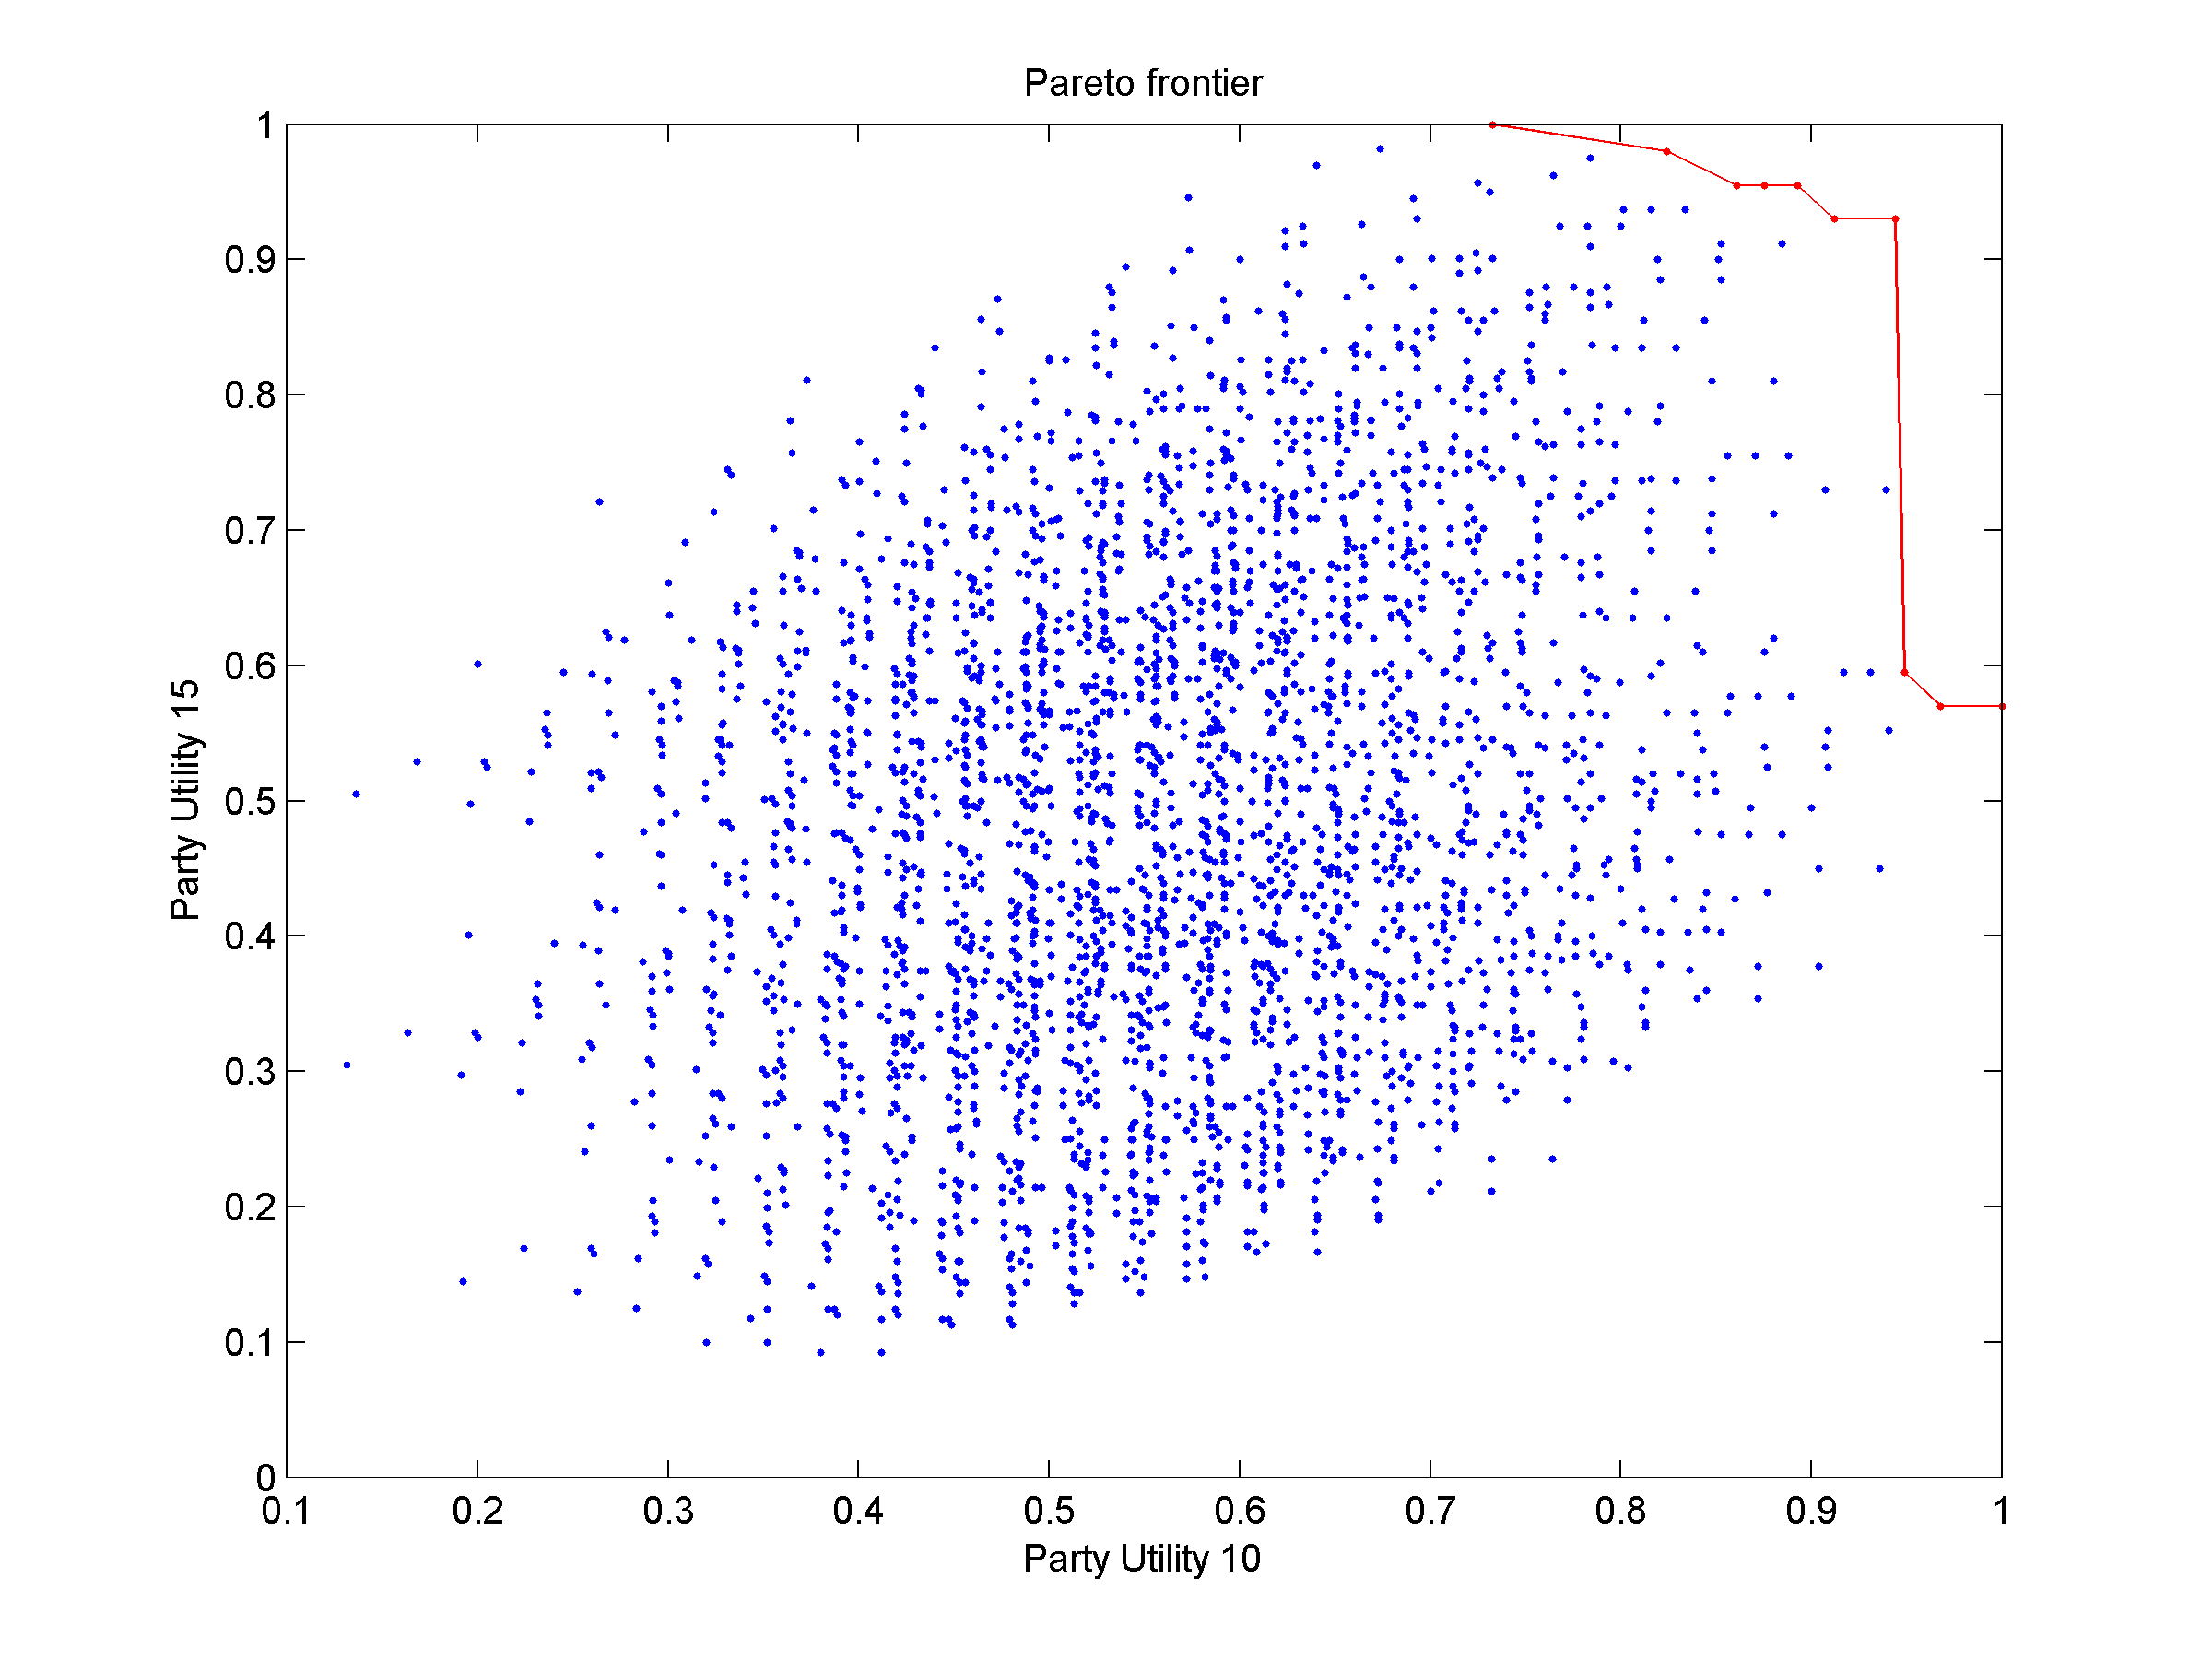
\includegraphics[width=0.6\textwidth]{pareto.png}
% \caption{The pareto optimal frontier is displayed with a red line in this figure.}
% \label{fig:pareto} 
\end{center}
%\end{figure}

\subsubsection{Analyse simple opponents}

Finally, we perform two negotation sessions: we play with the agent SimpleAgent against
itself, and we play Boulware vs. Conceder and explain the outcome.

\subsection{PEAS Description}

The first step in designing an agent is to specify the environment as fully as possible. In order to do this we specify the PEAS description which lists the following aspects of the environment: \emph{Performance}, \emph{Environment}, \emph{Actuators} and \emph{Sensors}. This measure is extensively discussed in Russel and Norvig \cite{russel-norvig}, so we adapt their notation.

\begin{table}[H]
    \begin{tabular}{|p{1.8cm}|p{3cm}|p{3cm}|p{3cm}|p{3cm}|}
    \hline
    \textbf{Agent} & \textbf{Performance \mbox{Measure}} & \textbf{Environment} & \textbf{Actuators} & \textbf{Sensors} \\
    \hline
    OurAgent & Own discounted utility at the end of the negotiation session & Negotiation space defined by Genius & Java classes that offer new bids to the opponent and the possibility to \mbox{accept/reject} offers & Java classes that return the bidding history of the \mbox{opponent} agent \\
    \hline
    \end{tabular}
    
    \caption{PEAS decription for our negotiation agent \label{table:peas-description}}
\end{table}

Table~\ref{table:peas-description} displays the PEAS descrition for our agent. We will briefly discuss each of the descriptions. First the \emph{environment} our agent operates in, this is the negotiation space as defined by Genius. \todo{Check the PEAS description I came up with and finish the additional description} 

\subsection{BOA Framework}

Most negotiation agents consist of three components: \emph{Bidding strategy}, \emph{Opponent model}, \emph{Acceptance strategy}. Together these three components form the \emph{BOA framework}. As discussed by Baarslag et al., the advantages of seperating the components using this framework are threefold \cite{baarslag2012decoupling}. In designing our negotiation agent the most useful advantage was the fact that it allows for easily changing individual compontents and analyze the interaction between the components. Below we provide a small description for the three required components.

\begin{description}
  \item[Bidding Strategy] \hfill \\
  The bidding strategy is arguably the most important compontent. Its goal is to determine the next bid that is offered to the oponent. In determining the next bid the agent can interact with the opponent model to provice a suitable offer. Sometimes the negotiation sessions is split up in multiple phases and each of the phases uses a different bidding strategy.

  \item[Opponent Model] \hfill \\
  Learning the opponents behavior is essential in a good negotiation session. It allows for adapting to the way the other party provides its bids. In practice this works by estimating the opponents \emph{preference profile}, which is usually done by adapting \emph{Bayesian modelling} or \emph{frequency analysis}.

  \item[Acceptance Strategy] \hfill \\
  Negotiation sessions ideally end by reaching an agreement. The acceptance strategy decides whether the opponents offer should be accepted. A broad variety of acceptance strategies is available reaching from postponing acceptance until the last step and aiming at fast decisions.

\end{description}

\todo{In the subchapters per boa component, go into more detail about the strategy. We should include ``an explanation of the negotiation strategy, decision function for accepting offers, any important preparatory steps, and heuristics that the agent uses to decide what to do next, including the factors that have been selected and their combination into these functions.''.
I'd suggest we mention java method names here and not in the high level description}

\subsection{Bidding Strategy}
\label{sec:strategyBS}
In this section we discuss the bidding strategy implementation of our negotiation agent.

\subsubsection{Opening Bid}
Our agent starts by offering a bid with utility 0.9. \todo{Fix this}

\subsection{First Phase}
In the first phase of the negotiation session our agents performs some kind of offering random bids to the opponent.

\subsection{Second Phase}

\subsection{Third Phase}



\subsection{Opponent Model}
\label{sec:strategyOM}

\subsection{Acceptance Strategy}
\label{sec:strategyAS}

\subsection{Opponent Strategy Model}
\label{sec:strategyOMS}

\section{Testing \& Performance}
\label{sec:performance}
\todo{a section documenting the tests you performed to improve the negotiation strength of your agent. You must include scores of various tests over multiple sessions that you performed while testing your agent. Describe how you set up the testing situation and how you used the results to modify your agent.}

\section{Questions}
\label{sec:questions}

\subsection{Analysis of the Party Domain}

\begin{enumerate}[(a)]

\item{test}

\end{enumerate}


\subsection{Example Code}


Example of java code inclusion:
\begin{lstlisting}
public Action chooseAction () { Action action = null;
  try {
    if (actionOfPartner == null) {
      action = chooseRandomBidAction ();
    }
    if (actionOfPartner instanceof Offer) {
      Bid partnerBid = ((Offer) actionOfPartner).getBid();
    }
  } catch
    e.printStackTrace();
    action = new Accept(getAgentID()); // best guess if things go wrong.
  }
  return action; 
}
\end{lstlisting}

\section{Conclusion}
\label{sec:conclusion}
\todo{a conclusion in which you summarize your experience as a team with regards to building the negotiating agent and discuss what extensions are required to use your agent in real-life negotiations to support (or even take over) negotiations performed by humans.}
As a conclusion I'd like to cite: \cite{baarslag2012decoupling}...

\subsection{Example Code}
Example of java code inclusion:

\begin{lstlisting}
public Action chooseAction () { Action action = null;
  try {
    if (actionOfPartner == null) {
      action = chooseRandomBidAction ();
    }
    if (actionOfPartner instanceof Offer) {
      Bid partnerBid = ((Offer) actionOfPartner).getBid();
    }
  } catch
    e.printStackTrace();
    action = new Accept(getAgentID()); // best guess if things go wrong.
  }
  return action; 
}
\end{lstlisting}

\bibliography{negotiation_final_report}
\bibliographystyle{plain}

\end{document}
